
%(BEGIN_QUESTION)
% Copyright 2011, Tony R. Kuphaldt, released under the Creative Commons Attribution License (v 1.0)
% This means you may do almost anything with this work of mine, so long as you give me proper credit

Suppose you ran a ``scan'' diagnostic test on a globe-style control valve equipped with a DVC6200 positioner, and obtained the following {\it valve signature} plot:

$$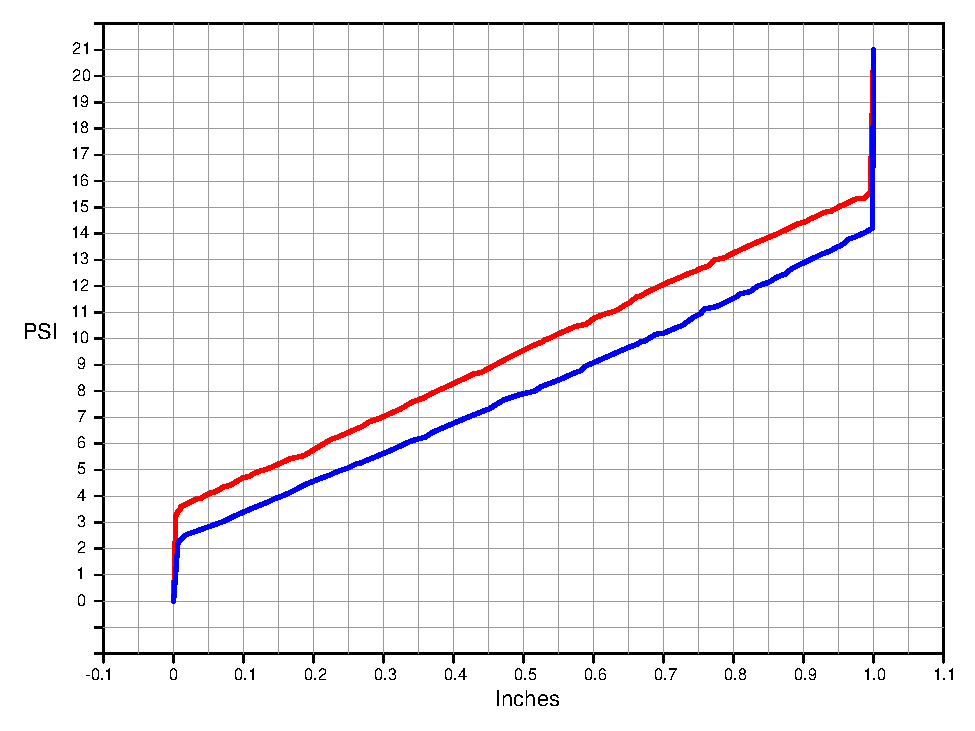
\includegraphics[width=15.5cm]{i00398x01.eps}$$

Based on this graph, estimate the maximum amount of frictional force the stem experiences while moving in each direction.  Assume a diaphragm actuator with a diameter of 13.9 inches.

\vskip 10pt

$F_{friction}$ = \underbar{\hskip 50pt} lbs

\vskip 10pt

Also, explain how the graph would become altered if the packing were lubricated to reduce friction, assuming stem packing is the main source of friction in this control valve mechanism.

\vskip 30pt

\underbar{file i00398}
%(END_QUESTION)





%(BEGIN_ANSWER)

5 points for a correct answer (within the given range), but only 1 point if the answer is double (i.e. the student did not divide the friction band by 2 when calculating):

\vskip 10pt

$F_{friction}$ = \underbar{\bf 113.81 to 151.75} lbs  {\it (depending where on the graph the values were sampled for the maximum friction calculation)}

\vskip 10pt

5 points for correctly assessing that the gap between the up and down trends would become {\bf narrower} if packing friction were reduced.

%(END_ANSWER)





%(BEGIN_NOTES)

{\bf This question is intended for exams only and not worksheets!}.

%(END_NOTES)


